% Preamble
\documentclass[a4paper,12pt]{article}

\usepackage[osf]{mathpazo} % palatino
\usepackage{ms}            % load the template
\usepackage[round]{natbib} % author-year citations
\usepackage{graphicx}      
\pagenumbering{arabic}    

% From Syst Biol template
\linespread{1.66}
\raggedright
\setlength{\parindent}{0.5in}

\pagestyle{empty}

\renewcommand{\section}[1]{
  \bigskip
  \begin{center}
  \begin{Large}
  \normalfont\scshape #1
  \medskip
  \end{Large}
  \end{center}
}

\renewcommand{\subsection}[1]{
  \bigskip
  \begin{center}
  \begin{large}
  \normalfont\itshape #1
  \end{large}
  \end{center}
}

\renewcommand{\subsubsection}[1]{%
\vspace{2ex}
\noindent
\textit{#1.}---}

\renewcommand{\tableofcontents}{}

\bibpunct{(}{)}{;}{a}{}{,}  % this is a citation format command for natbib

% Ignoring their title page setup as I like Rich's template better :)

% Title page information

\title{The ``Dark Side'' of Phylogenetic Comparative Methods}
\author{
  Richard G. FitzJohn$^{1}$, Cecile An\'{e}$^{2}$, Wayne Maddison$^{3}$,\\ Matthew W. Pennell$^{4}$, Gavin H. Thomas$^{5}$, April Wright$^{6}$,\\ and Natalie Cooper$^{7,8,*}$
}
\date{}
\affiliation{\noindent{\footnotesize
$^1$ Department of Biological Sciences, Macquarie University, Sydney, NSW 2109, Australia. \\
$^2$ Wisconsin\\
$^3$ UBC\\
$^4$ Institute for Bioinformatics and Evolutionary Studies, University
of Idaho, Moscow, ID 83844, U.S.A.\\
$^5$ Sheffield\\
$^6$ Austin\\
$^7$ School of Natural Sciences, Trinity College Dublin, Dublin 2, Ireland.\\ 
$^8$ Trinity Centre for Biodiversity Research, Trinity College Dublin, Dublin 2, Ireland.\\
$^*$ Corresponding author: ncooper@tcd.ie; Zoology Building, Trinity College Dublin, Dublin 2, Ireland. Fax: +353 1 677 8094; Tel: +353 1 896 1926.\\
}}

\vfill
%\paragraph{Word-count:} X words

\runninghead{The ``Dark Side'' of PCMs}
\keywords{PCM, assumption, etc.}

% End of preamble

\begin{document}
\modulolinenumbers[1]   % Line numbering on every line

\mstitlepage
\parindent = 1.5em
\addtolength{\parskip}{.3em}

%\section{abstract}
% If Syst Biol "Point of View" there's no abstract

\newpage
\raggedright
\doublespacing
%\section{Introduction} % No intro heading for Syst Biol

A long time ago in a galaxy far, far away - also known as the 1980s - phylogenetic comparative methods (PCMs) were developed to deal with the statistical non-independence of species in comparative analyses (e.g. \citealp{felsenstein1985phylogenies,grafen1989phylogenetic}). 
Since then PCMs have been extended to investigate evolutionary pattern and process, and include methods for investigating drivers of diversification, the tempo and mode of trait evolution, and models of speciation and extinction (see reviews in \citealp{o2012evolutionary, pennell2013integrative}). 
PCMs have become extremely popular over recent years; the number of papers featured the phrase ``phylogenetic comparative'' has increased exponentially since the 1980s (Figure \ref{PCMCitations}). 
With new methods being published almost weekly, there has never been a better time to be a comparative biologist.

\begin{figure}[h]
\centering
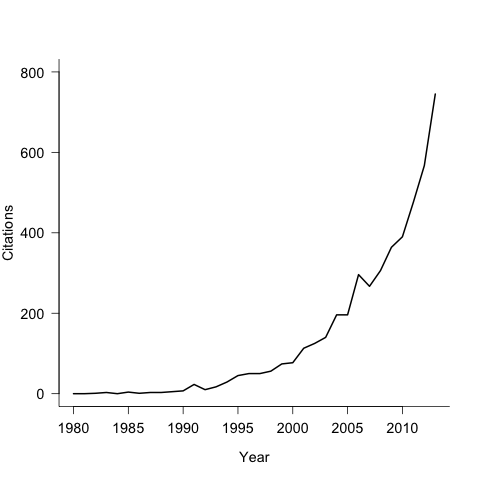
\includegraphics[width = 10cm]{PCMCitations.png}
\caption{PCM papers through time}
\label{PCMCitations}
\end{figure}

Unfortunately, PCMs also have a ``dark side''; they make various assumptions and suffer from biases in exactly the same way as any statistical method \citep{freckleton2009seven,boettiger2012your}. 
The more popular these methods become, the less awareness methods-users seem to have of this dark side. Increasingly assumptions and biases are inadequately assessed in empirical studies, leading to poor model fits and misinterpreted results. 
Additionally, little consideration is given to whether using a PCM is really appropriate for the question at hand \citep{losos2011seeing}. 
To paraphrase \citet{blomberg2012independent}, the enthusiastic application of PCMs has greatly outpaced our theoretical understanding of the methods and their relations to the rest of statistical theory.\\

% Do we need more explicit comments showing we're not the only people to think this, nor the first to say it?

One major issue is that two groups of people are involved with PCMs. 
At one extreme, methods-developers (``wookies'') develop new methods and implement them. They are (generally) aware of the limitations of their methods, and the assumptions that underly them. 
% Bit of a stretch but we can pretend right? :)
At the other extreme, na\"{i}ve methods-users (``ewoks'') just want to use PCMs to answer empirical questions with their data, and may not be aware of issues with the methods. 
Of course the majority of people fall somewhere between these two extremes on the ``wookie-ewok'' spectrum; many methods-developers are developing methods with a specific empirical question in mind, while there are many advanced methods-users who have detailed knowledge of the limitations of the methods they use. 
The problem is that although methods-developers (and advanced methods-users) are aware of the problems with PCMs, this information is not being effectively transferred to methods-users. Additionally, the tools and approaches used to fit models are often far more user-friendly and better documented than the methods used to to assess whether that model fit is reasonable. 
Clearly more effort is needed to bridge the widening gap between methods-users and methods-developers. Here we explore the causes of this communication gap and suggest some potential solutions. %still not happy with this writing

\section{What impedes information transfer from methods-developers to methods-users?}
% Or something similar

As scientists we mainly communicate our ideas and through the literature. Therefore, any difficulty transferring information between methods-developers and methods-users must begin with the literature. If this is the case we suggest three possible reasons:
%Yuk fix this

\begin{enumerate}
\item Not everything is mentioned in the literature.
\item The literature is too technical and/or important details are hidden within the text.
\item Methods-users have bypassed the literature and gone straight to the implementation of the method.
\end{enumerate}

%Note that we assume that methods-users ignore assumptions and biases because they are unaware of them. Of course, there may be methods-users who are perfectly aware of these issues but choose to sweep them under the carpet to get their work published. Although we believe there is no excuse for doing this, we also recognize that the ``publish or perish'' culture of academia may pressurize nontenured scientists into this. Hopefully some of the changes we suggest below will also help with this problem. 
%This could be a footnote, or left out!

\subsection{1. Not everything is mentioned in the literature}

A lot of the information needed to properly apply PCMs is not found in the literature. 
We refer to this knowledge as ``PCM folklore'' because it tends to be passed down from PIs to graduate students.
Sometimes the folklore includes tricks to get methods working, or useful rules-of-thumb. 
Other times folklore is more opinion-based, but over time these myths become set in stone. 
One example of such folklore is in the defaults of programs that perform PCMs. 
These often start out as arbitrary starting points for data exploration with no justification for their use, but over time become the way the analysis is always performed.
Useful PCM folklore is often shared among methods-developers, and among collaborating groups, but is rarely shared outside of these circles. 
When it is shared, it tends to be in the form of email exchanges between methods-developers and struggling methods-users.
This advice is extremely useful to the methods-user in question, but forms a kind of ``dark advice'' that isn't accessible to the rest of the community.\\

% Do we want a specific example here? Theta estimation in OU models? 
% Could mention ±3 from Jones&Purvis97 - totally unjustified rule of thumb now = canon.
% Mention hidden assumptions?

Other information about the limitations of a method may be absent from the literature due to the time lag between a new method being published and others having time to test and critique it. 
For example, \citet{felsenstein1985phylogenies} published the phylogenetic independent contrasts method in 1985, but it wasn't until the early 1990s that real critiques of the method and its assumptions began to be published. %add citations.
This time lag is shorter with more recent methods because simulations testing the method are now required by journals.
However, we suspect there are still many hidden assumptions and biases in virtually all PCMs.

\subsection{2. The literature is too technical and/or important details are hidden}

Although a lot of information is not found in the literature (see above), the majority of assumptions and biases of PCMs are documented somewhere. 
A big issue for novice methods-users is that this information is often extremely technical and dense.
It is not unusual for papers to be full of equations, over 20 pages long, and written in a way that gives even advanced users a headache. 
Additionally there is a lot of literature to wade through before getting all of the required information. 
For example, one of us (NC) recently reviewed papers discussing the assumptions and limitations of the most commonly used PCM, phylogenetic independent contrasts \citep{felsenstein1985phylogenies}. 
Even with prior knowledge of the key papers and authors to focus on, this resulted in XX pages, XX papers and a book to read. 
This seems like an excessive amount of reading to expect from a methods-user trying to run a simple empirical analysis.\\

Another issue is that it can sometimes be hard to find the information required. Assumptions and caveats can be found in the Introduction, Methods, Results and/or Discussion of a paper. 
They are rarely neatly corralled in one place, making it really easy to miss pertinent details. 
This places an additional burden on methods-users who must read every paper very carefully.

\subsection{3. Users jump straight to the implementation of the method}

In the early days of PCMs there was


Increasingly new PCMs are published with an accompanying R package, or at least some code


%This increase in use is at least partially the result of the number of available R packages to run these analyses (for example ape, GEIGER, diversitree, caper - citations) and the community's increasing familiarity with R \citep{R-Core-Team:2014aa}. Unfortunately with this increase in popularity, comes an increase in misuse! % need to work on this paragraph

%Huge increase in number of PCM packages since 1980s, and especially since 2008 [Graph]. Now people familiar with R they can just jump in and try stuff on their data with very little knowledge of what is going on or what the results mean [Though code sharing is cool and I’m not dissing that]. 

%I’m torn as to what I think here – part of me thinks there should be a mention of assumptions in the manual/vignette (though not if this replicates an accompanying blog or book or something) but part of me thinks it’s the users responsibility to not be a fuckwit. Caper, diversitree and CAIC are good examples where assumptions are clearly laid out and methods for testing assumptions are available in caper and CAIC (not sure about diversitree ...). Ape book has none of this in it at all!

%Again this needs to be incentivized as it’s adding work for already hard working and underappreciated methods developers. Funding of pure methods to encourage methods developers to make methods more user friendly, and to take the time to add methods for detecting deviations from assumptions rather than rushing to publish.

\section{How can we solve some of these problems?}

\subsection{1. Simplify, summarize and share}
\subsection{2. Read, think and learn}
\subsection{3. Collaboration}
\subsection{4. Incentives}

%Such issues are the responsibility of end users but also of methods developers: the tools and approaches used to fit models are often far more user-friendly and better documented than the methods used to to assess whether that model fit is reasonable. To address these issues, we propose this symposium to discuss issues in both classical and recent PCMs, along with new research on detecting for these issues and accounting for them.  We hope that this will both increase awareness of these problems and encourage further research and careful thought in the area, along with better dialogue between method developers and method users.

%Big issue = who is responsible? Can't expect empiricists to be an expert in every method, but do want to add to workload of overloaded developers.

%Improvements in methods, and ways of detecting biases etc should be sufficient for publication (rather than MEE's weird focus on novelty now it has a huge IF)

%Incentives - funding for pure methods. Different authorship rules. 

%Change the definition of success in academia. Quality not quantity. Remove rush to publish. This would help WOMEN too!

%Collaborate! But make collaboration valuable to non first authors somehow

%We really *do not* want to lose all the technical people from science. We need them more than ever as evo bio becomes more and more computationally intensive. Need to make it worth their while (can't match wages of industry)

%Add methods to test assumptions as standard to packages. 

%Grouping assumptions, biases and caveats more carefully in papers. Caveats box???

%Accompanying blogs with methods papers to explain to non-technical audience. Could be Supp Matt too. Lavin et al 2008 is a beautiful example.

%Some website with a list of key papers, and key summary points, for each method. Who would host? Who would write? Who would peer review?

%Users need to take responsibility too. Work harder to understand. Read widely. Don't take results at face value. Become less trusting! Simulate data to check method does what you think it should do. Don't be afraid to question standard practice - sometimes it's just folklore. My pglm vs pgls example.

%Can we expect methods users to read every paper before using a method? (Yes – wouldn’t let someone work on your microscope unless you were sure they knew what they were doing!!!). Perhaps some work to be done in summarizing this – needs incentives – no benefits to wikis and workshop teaching cf to writing high impact papers, or papers at all. However, people willing to share skills are the people we really want as colleagues, not the selfish high achievers! Collaborate with someone who does know this stuff? Again problematic as highly skilled technical people end up with too much to do and still end up only being middle author. Maybe something like in physics with “theoretical lead” and “technical lead” authors??? Perhaps write a less technical summary for methods papers, or a “Caveats box” to put this up front – i.e. will only work if you have X taxa and this kind of data. Check these assumptions. Incentivize accompanying blogs to explain this stuff? Funding of pure methods to encourage methods developers to make methods more user friendly, and to take the time to add methods for detecting deviations from assumptions rather than rushing to publish. Speed up publication by archiving. Put code on github so knowledgeable users can access at an earlier stage if they want to. Helpful for finding bugs etc. Methods developers could also benefit from collaboration with methods users who could help them find corner cases and make their methods more useful with real data? [Again I’m torn with some of these ideas because is it really the developer’s job to stop people from being fuckwits? But if this info isn’t included here, *where* would it come from and *who* would provide it? Users can’t be trusted.]

%A New Hope joke...

\section{Funding}
This work was supported by The European Commission CORDIS Seventh Framework Program (FP7) Marie Curie CIG grant, proposal number: 321696 (NC). 

\section{Acknowledgments}
Thanks to the Society of Systematic Biologists for funding our symposium at Evolution 2014. We also thank George Lucas for the ``hilarious'' Star Wars jokes.

\bibliographystyle{sysbio}
\bibliography{darkside}

\end{document}
